\lecture{Tue. 9/11/12}

Today, Bill Minicozzi is teaching again.

We define tangent bundles and vector spaces on manifolds, and then define the Lie derivative---the analogue of a derivative for vector fields. We'll derive basic properties of the Lie derivative, and understand why it is a natural thing to consider.

\subsection{Tangent bundle}

%A vector $v\in T_pM$, $p\in M$ is $v:\cal D\to \R$
%
%Don't nec know how to work, but well-defined. 
%
%In local coordinates, satisfy a certain transformation law, immediately know how to compute, but need to show well defined. Make sure make sense if do different coordinates

The \textbf{tangent bundle} is basically built from considering 
\begin{enumerate}
\item
all possible points, and
\item
all possible tangent vectors at that point.
\end{enumerate}
At each point the tangent space is like $\R^n$. We have a ntural basis for the tangent basis in a given chart; namely, taking partial derivatives with respect to the coordinates of the chart. We now give the formal definition.

\begin{df}
Let $M$ be a $n$-dimensional manifold. The \textbf{tangent bundle} $TM$ is a $(2n)$-dimensional manifold, defined as follows.
\begin{enumerate}
\item
As a set,
\[
TM=\set{(p,v)}{p\in M,\,v\in T_pM}.
\]
\item The charts are as follows. Start with the charts of $M$,  $x_{\al}:U_{\al}\to M$. Define
\[
y_{\al}:U_{\al}\times \R^n\to TM
\]
by
\[
y_{\al}(\underbrace{x_1^{\al},\ldots,x_n^{\al}}_{\text{in }U_{\al}},\underbrace{u_1,\ldots, u_n}_{\text{point in }\R^n})=
(x_{\al}(\underbrace{x_1^{\al},\ldots, x_n^{\al}}_{\text{point in }M}),\sum_{i=1}^n u_i\underbrace{\pd{}{x_i^{\al}}}_{\text{basis elements}})
\]
\end{enumerate}
\end{df}
This map is injective because $\pd{}{x_i^{\al}}$ are linearly independent basis elements. We need to check that the overlap properties work---this is standard and left to the reader.

At first glance, the tangent bundle does not seem to give much more info than $M$ itself. It looks like we're taking the product of $M$ with $\R^n$. In fact, we can contract $TM$ to $M$, by contracting each set $\{p\} \times T_pM$ to just $\{p\}$.

But often $TM\ne M\times\R^n$. We get extra information because the tangent bundle can ``spin around." When we trace out a loop in $M$, the tangent space might spin around completely once---so we get some nontrivial topology here. 

For example, consider the tangent bundle of $S^1$. At each point, the tangent space is $\R$, and it turns out that the tangent bundle is a cylinder (exercise),
\[TS^1=S^1\times \R.\]
However, if the tangent bundle had ``spun around," then we would get a M\"obius band instead.

For those in the know, the tangent bundle is a special case of a {\it fiber bundle}. (We won't cover this more general notion, so that we can get more quickly to the geometry. But if you're interested, see~\url{http://en.wikipedia.org/wiki/Fiber_bundle}.)

\subsection{Vector fields}

We can now generalize the definition of a vector field to an arbitrary manifold.

\begin{df}
A (smooth) \textbf{vector field} $X$ on $M$ is a map taking each point $p\in M$ to $X(p)\in T_pM$, such that the map $M\to TM$ induced by this map sending $p\mapsto (p,X(p))$ (the fiber above the point) is smooth.
%sending each point to a fiber above that point.
\end{df}
We can also talk about continuous, $C^1$, etc. vector fields, in which case we replace the ``smooth" condition by the appropriate condition.

%section of a bundle. 
%no fiber bundles- quickly get into geometry

In a chart, we can write
\[
X(p)=\sum_{i=1}^n a_i(p)\pd{}{x_i}.
\]%smooth functions of p; basis vf's
The fact that $X$ is smooth is equivalent to all the $a_i(p)$ being smooth. We get a function $X:\cal D\to \cal D$ (recall $\cal D$ is the space of smooth functions $M\to \R$) that operates as
\[
Xf=\sum_{i=1}^n a_i\pd{f}{x_i}
\]
where implicitly at each point $p$ we take a chart containing $p$.

Since $X$ gives a tangent vector for each point of $M$, it allows us to take directional derivatives at each point.
We call $Xf$ the derivative of $f$ with respect to $X$. Note that $X$ is a derivation: it is $\R$-linear ($X(fg)=Xf+Xg$, $X(af)=aXf$) and satisfies the Leibniz rule ($X(fg)=(Xf)g+f(Xg)$).
%Tangent vectors at each point allow us to take directional derivatives at each point.

\subsection{Lie derivatives}

We've saw how to take the derivative of a function on the manifold with respect to a vector field. Now we would like to take the derivative of vector field {\it with respect to another vector field}, but we have a problem. Let $X$ and $Y$ be vector fields on $M$. Can we take a directional derivative of $Y$ in direction $X$? Suppose we wanted to take
\[
\lim_{t\to 0} \fc{Y(p+tX)-Y(p)}{t}.
\]
This is roughly what the derivative should be. Our first problem is that this is just for Euclidean space, rather than general manifolds. For a general manifold, letting $\al$ be a curve $\al:(-\ep,\ep)\to M$, and supposing $\al(0)=p$, $\al'(0)=X(p)$, we can try to define
%can define a flow, look at curve tangent to X 
\[
\lim_{t\to 0} \fc{Y(\al(t))-Y(p)}{t}
\]
However, {\it $Y(\al(t))$ and $Y(p)$ do not live in the same vector space}: $Y(\al(t))$ lives in $T_{\al(t)}M$ and $Y(p)$ lives in $T_p(M)$. %no go

We are stuck unless we find a canonical way to identify these vector spaces!

There are two different ways to identify these spaces. 
\begin{enumerate}
\item
The first way is the Lie derivative, which we'll cover today. The idea is to integrate the vector field to get a diffeomorphism on the manifold, which allows us to move one point to another point. Recall that a smooth map $\ph:M\to N$ induces a differential sending the tangent space of the first point to the tangent space of the second point, $d\ph_p:T_pM\to T_{\ph(p)}N$. We can go back as well, since we have a diffeomorphism.
\item 
The second way is to equip the manifold with extra structure, called a Riemannian connection. We use parallel transport to identify vector spaces of different points. We get what is called the covariant derivative. 
\end{enumerate}

%flow

\subsubsection{Lie derivative (bracket)}
\begin{df}
Define the \textbf{Lie derivative (Lie bracket)}
$[X,Y]=L_XY$ by
\[
[X,Y]f:=X(Y(f))-Y(X(f)).
\]
\end{df}
From this definition it is not obvious that this is the ``derivative" of anything; this will be clear after we derive an alternate expression for it.

Note that we're differentiating $f$ twice, so the Lie bracket depends on at most 2 derivatives of $f$; it is sufficient for $f$ to be $C^2$. %a priori %leibniz rule. 
In fact, $[X,Y]$ depends only on the first derivatives of $f$ and is itself a vector field. 

In a chart, we can write
\bal
X&=\sum_{i=1}^n a^i\pd{}{x_i}\\
Y&=\sum_{i=1}^n b^j\pd{}{x_j}.
\end{align*}
We calculate, using the product rule,
\bal
X(Y(f))&=X\pa{\sum_{j=1}^n b^j\pd{f}{x_j}}
=\sum_{i,j} a^i\pa{{\color{blue}b^j\pd{^2f}{x_j\partial x_i}}+\pd{b^j}{x_i}\pd{f}{x_j}}\\
Y(X(f))&=Y\pa{\sum_{i=1}^n a^i\pd{f}{x_j}}
=\sum_{i,j} b^j\pa{{\color{blue}a^i\pd{^2f}{x_i\partial x_j}}+\pd{a^i}{x_j}\pd{f}{x_i}}
\end{align*}
When we subtracting, the first terms (in blue) cancel, because partial derivatives in Euclidean space commute. We switch $i$ and $j$ in the second terms and compute
\begin{align}
\nonumber
[X,Y]f&=\sum_{i,j} a^i \pd{b^j}{x_i}\pd{f}{x_j}-\sum_{i,j}b^i\pd{a^j}{x_i}\pd{f}{x_j}\\
\nonumber
&=\sum_{j=1}^n\ba{\sum_{i=1}^n\pa{a^i\pd{b^j}{x_i}-b^i\pd{a^j}{x_i}}\pd{f}{x_j}}\\
\llabel{eq:18965-2-1}
[X,Y]&=\sum_{j=1}^n \ba{\sum_{i=1}^n\pa{a^i\pd{b^j}{x_i}-b^i\pd{a^j}{x_i}}\pd{}{x_j}}
\end{align}
%all infinitely diff'ble. C^2 enough.
In the Euclidean case, we have found a formula for $[X,Y]$.
For the general manifold, we are also done, but we should say a few more words. Equation~\eqref{eq:18965-2-1} gives a formula in one chart.

What if write it in another chart; do we get the same vector field? In other words, do we get the same result if we computed~\eqref{eq:18965-2-1} for a different chart, and if we compute~\eqref{eq:18965-2-1} in the first chart and then use the Jacobian to change coordinates?  Yes, because the Lie bracket is uniquely defined by $[X,Y]f=XYf-YXf$. %diff expres. Jacobian formula, forced on us, same if Jac move? Only thing can get, b/c bracket def in unique vf. Unique vf, b/c basis.
%I'M CONFUSED BY THIS.

If the vector field is a coordinate vector field, i.e. the $a_j$ and $b_j$ are constants, then the Lie bracket is 0. For a vector field coming from any coordinate system, the Lie bracket is always 0. In a sense the Lie derivative measures the obstruction to coordinates existing.
\subsubsection{Properties of $[,]$}
\begin{pr}
Thie Lie bracket satisfies the following.
\begin{enumerate}
\item
(Anti-commutativity) $[X,Y]=-[Y,X]$
\item
($\R$-linearity) $[X,aY+bZ]=a[X,Y]+b[X,Z]$.
\item
(\textbf{Jacobi identity}) %cyclically permute and add up get 0.
$[[X,Y],Z]+[[Y,Z],X]+[[Z,X],Y]=0$ (If you cyclically permute $[[X,Y],Z]$ and sum, you get 0.
%st deeper
%for lie algebra
%in what way are vf a lie algebra
%grp of diffeomoetrphism
%tangent space at identity given by integratin vf.
%to grp of diffeo.
%lie alg is set of groups.
%bracket is bracket for lie group
%where this comes from (not prove)
\item
$[fX,gY]=fg[X,Y]+fX(g)y-gY(f)X$.
\end{enumerate}•
\end{pr}
As we'll explain after the proof, the Jacobi identity has a deeper reason for being true.
\begin{proof}
\begin{enumerate}
\item
We have $[X,Y]=X(Y(f))-Y(X(f))=-(Y(X(f))-X(Y(f)))=-[Y,X]$.
\item
Taking derivatives is linear. %, derivative kills constants. (Or see from formula)
\item Expand out each bracket, and add them all up. We have %4 terms from each, 12 terms, 6 with +, 6 with -, all cancel.
\bal
[[X,Y],Z]f&=[X,Y]Z(f)-Z([X,Y]f)\\ %only 1 order make sense do these things\\
&=XYZ(f)-YXZ(f)-ZXY(f)+ZYX(f).\\
\implies [[X,Y],Z]&=XYZ-YXZ-ZXY+ZYX\text{ (in shorthand)}
\end{align*}%{\color{blue}
Cyclically permuting $X\mapsto Y \mapsto Z\mapsto X$, 
\bal
[[Y,Z],X]&=YZX-ZYX-XYZ+XZY\\
[[Z,X],Y]&=ZXY-XZY-YZX+YXZ.
\end{align*}
We find that all 6 permutations of $X$, $Y$, and $Z$ occur, 6 of them are positive, and 6 of them are negative. Thus adding the 3 brackets gives 0.
\item First we find $[X,gY]$. We go nuts with the Leibniz rule, calculating
\begin{align}
\nonumber
[X,gY](h)&=X(gY(h))-gY(X(h))\\
\nonumber
&=X(g)Y(h)+gX(Y(h))-gY(X(h))\\
\nonumber
&=X(g)Y(h)+g[X,Y]h\\
\implies  [X,Y]&=X(g)Y+g[X,Y].\llabel{eq:18965-2-2}
\end{align}
We have a similar formula for $[fX,W]$.
\begin{equation}
[fX,W]=-[W,fX]=-W(f)X-f[W,X]=-w(f)X+f[X,W].
\llabel{eq:18965-2-3}
\end{equation}
Putting~\eqref{eq:18965-2-2} and~\eqref{eq:18965-2-3} together gives
\bal
[fX,gY]&=-gY(f)X+f\underbrace{[X,gY]}_{X(g)Y+g[X,Y]}\\
%&=-gY(f)X+f()\\%tedious, but get feel for how work. %``I get to struggle with it on the board."
&=-gY(f)X+fX(g)Y+fg[X,Y]
%1/8 chance match other formula MIRACLE
\end{align*}
\end{enumerate}
\end{proof}
%We are adding more and more layers of structure for manifolds. %Today Riemannian strucutre (measure) too.
We proved the Jacobi identity with computation; there's a more general reason why it's true.

\subsubsection{Flows and the Lie derivative}

Let $X$ be a vector field in $M$. Imagine if we were to start at some point $p$ at the manifold, and then at every instant in time, go in the direction given by the vector field. The vector field tells us how to ``flow." We would trace out a curve starting at $p$, whose tangent vector everywhere is the vector field. We can think of this ``flow" happening everywhere on the manifold, i.e. the whole manifold is ``flowing." The curves that are traced out at different points will not cross.
% look at flow lines. Curve starts at that point, tangent vector everywhere is vector field. 
%nice pics. Don't cross.

Formally, given $p\in M$, we want some curve $\al_p(t)$ such that 
\bal
\al_p(0)&=p\\
\al'_p(t)&=X(\al_p(t)).
\end{align*}
\begin{thm}[Existence and uniqueness of solutions]\llabel{thm:odes}
There exists a unique solution $\al_p(t)$ in some interval $(-\ep,\ep)$. Moreover, $\al_p(t)$ is a smooth function (with respect to $(p,t)$) defined on some open set in $M\times \R$ containing $M\times \{0\}$.
%First-order linear ODE: existence and uniqueness of solution, and smooth dependence on initial conditions
\end{thm}
\begin{proof}
Take a coordinate chart, and appeal to the existence theorem for ODE's in Euclidean space. (See Theorems 4.3-5 in Guillemin's 18.101 notes.)
\end{proof}
(Note: if $M$ is compact, then $\al_p(t)$ is defined for all $t\in \R$.)

%specified tangent vectors
Smooth dependence on initial conditions tells us that we can think of $p$ as another parameter. We thus write
\[
\ph(p,t):=\al_p(t).
\]

%ode theory
%Thus the map $\ph(p,t)$, $\ph:U\times (-\ep,\ep)\to M$ is \textbf{smooth}. $U$ open set in $M$. 
\begin{pr}
We have the following properties for $\ph$.
\begin{enumerate}
\item
$\ph(p,0)=p$.
\item
$\ph(p,s+t)=\ph(\ph(p,s),t)$.
\item Each map $\ph(\bullet t)$ is locally invertible. The inverse to $\ph(\bullet,t)$ is $\ph(\bullet,-t)$. %if flow from time t: p to $\al_p(t)$
%flow backwards for time t_0, get back where started. 
%flowing forwards for time t is the same as flowing backward for time t.
\end{enumerate}
\end{pr}
We encapsulate these conditions with the following statement.\\

\cpbox{
$\ph(\bullet,t)$ is a \textbf{1-parameter family} of (local) diffeomorphisms with $\ph(\bullet, 0)=\id$. The tangent at 0 is just the vector field.}
\vskip0.15in

Thus we see that $\ph(\bullet,t)$ (thought of as a function of $t$, whose output is a function on the manifold) is a path in the space of diffeomorphisms. It goes through the identity at $t=0$, and its tangent space is given by the vector field. Thus, the vector field is the Lie algebra associated to the Lie group of diffeomorphisms. The Jacobi identity holds in any Lie algebra. Thus it comes from something deeper, and is not just a miracle with 6 positive and 6 negative terms. (Don't worry if you don't understand this.)
\begin{proof}
\begin{enumerate}
\item By definition.
\item This follows from uniqueness for ODE's (Theorem~\ref{thm:odes}) and reparameterizing. 
\item
Follows from part 2. Think of this as ``reversing time." %find it is also the soolution 
\begin{center}
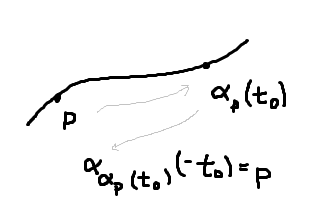
\includegraphics{2-1}
\end{center}
\end{enumerate}•
\end{proof}
%Can think of 1-parameter of maps from $U$ to $M$. At 0 get identity map.

%Whole manifold moving with flow. No longer identity.

%cpt no problem 
\begin{rem}
%Note get on $(-\ep,\ep)$ basically by smooth dependence on initial conditions. 
Note that solutions may blow up in finite time. For example, consider $\al(t)$ on $\R$ starting at 1, satisfying
\bal
\al(0)&=1\\
\al'(t)&=X(\al(t))=\al^p(t).
\end{align*}
We have 
\bal
(\al^{1-p})'&=(1-p)\fc{\al'}{\al^p}=(1-p)%\\
%(\al^{1-p})'&=-C
\end{align*}
Since the RHS is constant, we have $\al^{1-p}\to 0$ in finite time, and $\al$ blows up when $p>1$.

%p>1 
There is no uniform interval $(-\ep,\ep)$ that works for every point; $\ph$ is not globally defined on $\R$ for any $p>1$. However, if $\al$ is initially in a finite neighborhood of 0, it will be defined for some period of time $(-\ep,\ep)$. Given a time interval, there is a small enough neighborhood in $M$ where $\ph$ is defined.
\end{rem}
%tip: Never ever pick a word problem haven't done at board in class of >3 people. So people. So now we see we get a problem...

%Set
%\[
%\ph_t(p)=\ph(p,t).
%\]
%This is generated by $X$. 
We can now see in what sense the Lie derivative is a ``derivative," by relating it to $\ph$.
\begin{pr}
Let $\ph_t$ be the local flow of $X$. Then
\[
[X,Y]=-\left.\fc{d}{dt}\right|_{t=0}d\ph_{-t}(Y)\circ \ph_t.
\]
\end{pr}
In other words,
\[
([X,Y]f)(p)=-\left.\fc{d}{dt}\right|_{t=0}d\ph_{-t}(Y)f(\ph_t(p)).
\]
\begin{proof}
See do Carmo,~\cite[Prop. 5.4, p. 28]{dC}.
%\fixme{I don't think I quite have this right... FIX ME.}
\end{proof}

\cpbox{
In order to define the derivative of a vector field with respect to another vector field, we need a way to identify different tangent spaces. The Lie derivative is one such way; it identifies tangent spaces using the flow $\ph_t$ of the vector field.
}
\vskip0.15in
%use $\ph_t$, flow to move vector fields. Connects lie bracket with diffeo. 
%0 if Y does not move along the flow. Coor vect field 0. Constant translation in space. Not changing vf assoc to coordinate functions. 
We'll make 2 assumptions from now on: Manifolds are  ``nice" in the following sense.
\begin{enumerate}
\item
Hausdorff: Given $p \ne q$, there exist open sets $U_p$, $U_q$ such that $p\in U_p$ and $q\in U_q$ such that $U_p\cap U_q=\phi$.
\item Countable basis: $M$ is covered by a countable collection of coordinate charts. %partitions of unity.
\end{enumerate}•
